\documentclass{article}
\usepackage{graphicx}
\usepackage{float}
\usepackage{subcaption}
\usepackage{amsmath}
\usepackage[final]{pdfpages}
\usepackage{hyperref}
\usepackage{titlesec}
\usepackage{caption}
\usepackage{appendix}
\captionsetup[figure]{labelformat=empty}
\hypersetup{
colorlinks,
citecolor=black,
filecolor=black,
linkcolor=black,
urlcolor=black
}
\titlespacing*{\section}{0pt}{1cm}{0.5cm}
\titlespacing*{\subsection}{0pt}{0.5cm}{0.5cm}
\title{Travlendar+\\Acceptance Test Delivery}
\author{Fumagalli Paolo, Grotti Pietro, Gullo Marco}

\begin{document}
\pagenumbering{gobble}
\begin{figure}[t]

\includegraphics[width=\linewidth]{Images/Logo_Politecnico_Milano.png}
\label{fig:Logo}
\end{figure}
\maketitle

\newpage
\pagenumbering{roman}
\tableofcontents
\newpage
\pagenumbering{arabic}
	\section{Introduction}
		\subsection{Purpose}
			\paragraph{}The following document aims at showing the Acceptance Testing results of the analysis our team conducted on team D’ Amico - Gabbolini - Parroni’ s project. We were asked to go through all the documents that team has produced ( RASD, DD and ITD) and verify the if their first prototype of the application was coherent with them.    
		\subsection{Scope}
			\paragraph{}We could not find inconsistencies between the RASD and the DD, that appeared very well related. ITD fitted perfectly in the project context as well.\\Our team decided to focus on verifying the goals and requirements that the other team claimed to have successfully implemented, checking if errors or anomalies occurred.\\Some acceptance test cases were executed, one case for each goal: in Acceptance Test Results  section it is possible to see if any trouble came out in the mobile version (.apk file) provided. 

	\section{Group Identification}
		\subsection{Authors}
		\begin{itemize}
			\item{} Edoardo D'Amico
			\item{} Giovanni Gabbolini
			\item{} Federico Parroni
		\end{itemize}
		\subsection{Repository}
		\paragraph{} \href{https://github.com/keyblade95/DamicoGabboliniParroni/}{https://github.com/keyblade95/DamicoGabboliniParroni/}
		\subsection{Reference Documents}
		\begin{itemize}
			\item{}RASD: Requirement Analysis and Specification Document, Version 1.1 
			\item{}DD: Design Document, Version 1.1
			\item{}ITD: Implementation and Test Deliverable, Version 1.0
		\end{itemize}
\newpage
	\section{Installation Instructions}
		\paragraph{} To install the software we had to download an APK from a dropbox folder provided in their ITD. The APK worked as expected, we installed the application in three different devices, a Samsung Galaxy S8, a Sony Xperia Z3 Compact and a Huawei P8 Lite 2017 and tested the application with these phones. 
\newpage
	\section{Acceptance Test Cases}
		\paragraph{}Here are shown all the cases we believed as most relevant in the implementation evaluation. All the pictures below are extracted from their ITD.   
		\subsection{Server Side}
			\subsubsection{Registration}
			\begin{figure}[H]
			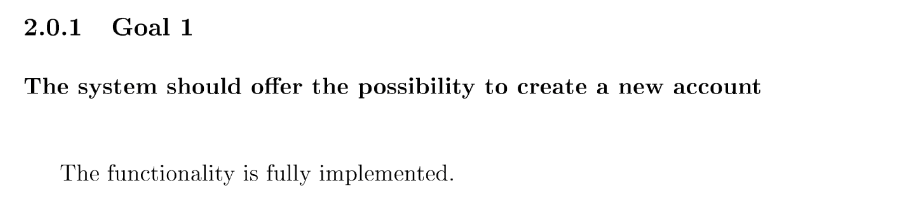
\includegraphics[width=\linewidth]{Images/Goals/Goal_1.png}
			\label{fig:G1}
			\end{figure}
			\paragraph{}We tested the registration by inserting a valid email address and a password. The result came as expected, the account was successfully created.\\
We also tried to register with an already used email address and the application didn’t allow us to register, as it would be expected, because the email was already used.\\
Future development tip: the client application should wait for the server to notify the registration result, without allowing the user to type anything in the registration form.
\newpage
			\subsubsection{Login}
			\begin{figure}[H]
			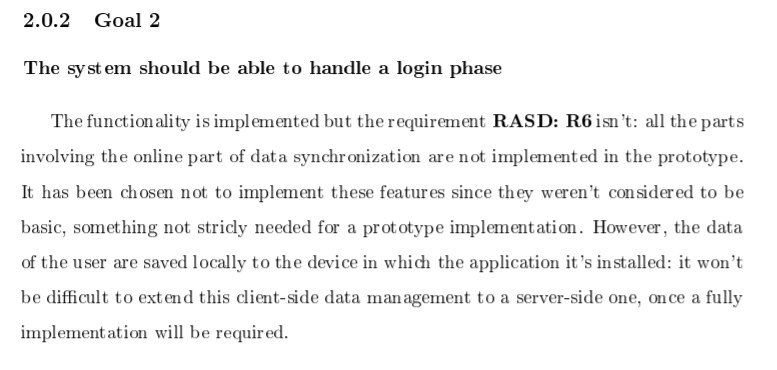
\includegraphics[width=\linewidth]{Images/Goals/Goal_2.jpg}
			\label{fig:G2}
			\end{figure}
			\paragraph{}The login was also successful. We tried to login with the same account on different devices and it worked, which means that the accounts are stored on the server database, but, as stated by the developers in the ITD, the appointments loaded on the application are the ones saved on the client, which means that logging from the same phone with different accounts loads the same appointments.\\ We also tried to insert the wrong information in the login form and the application notified us with an error message, as expected.
\newpage
		\subsection{Client Side}
			\subsubsection{Password Recovery}
			\begin{figure}[H]
			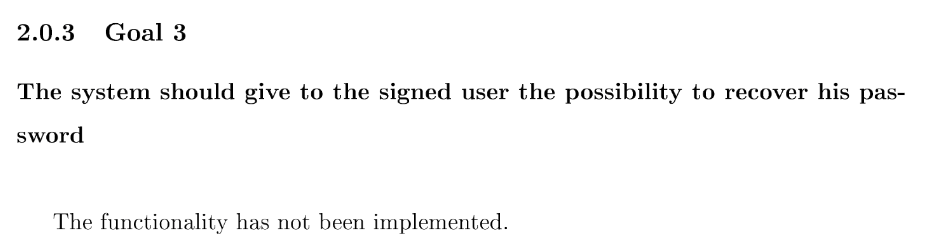
\includegraphics[width=\linewidth]{Images/Goals/Goal_3.png}
			\label{fig:G3}
			\end{figure}
			\paragraph{}This goal is not implemented, as stated in the ITD.
			\subsubsection{Appointment Creation}
			\begin{figure}[H]
			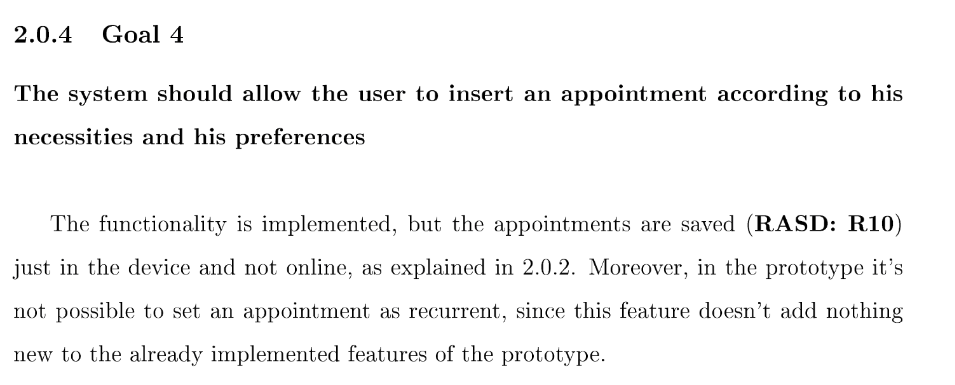
\includegraphics[width=\linewidth]{Images/Goals/Goal_4.png}
			\label{fig:G4}
			\end{figure}
			\paragraph{}The appointments are successfully created if you create an event which starts at a feasible time. The location search works perfectly and the form is well structured. If you try to insert an appointment which starts before the local time the application will crash instead of sending an error notification. It also sometimes crashes if you forget to input how many people are involved in the event.
			\subsubsection{Editing An Appointment}
			\begin{figure}[H]
			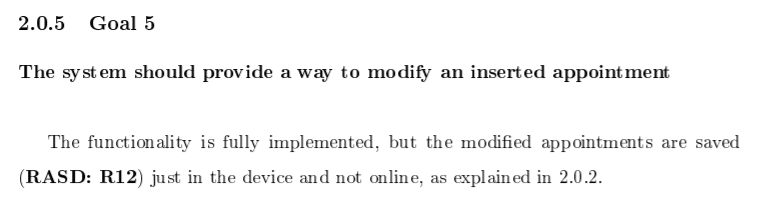
\includegraphics[width=\linewidth]{Images/Goals/Goal_5.png}
			\label{fig:G5}
			\end{figure}
			\paragraph{}We tried to edit multiple appointments and it always worked without problems. 
			\subsubsection{Schedule Creation}
			\begin{figure}[H]
			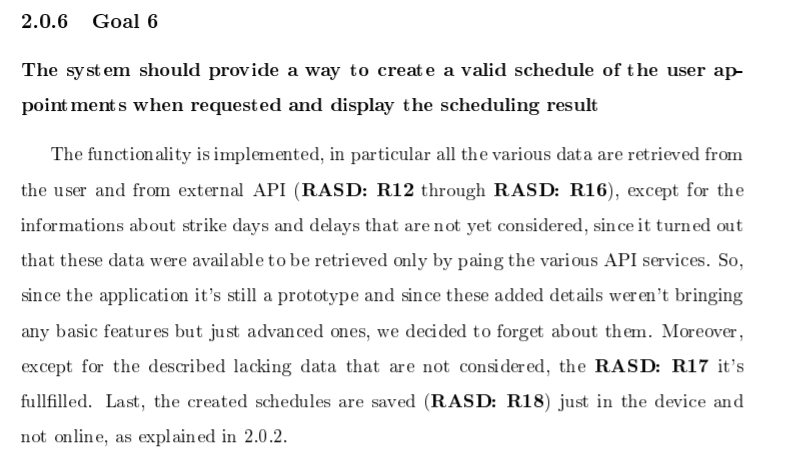
\includegraphics[width=\linewidth]{Images/Goals/Goal_6.png}
			\label{fig:G6}
			\end{figure}
			\paragraph{}The schedule creation works but has some problems. For example, if a schedule is not feasible the application simply notifies the impossibility of creating a schedule, without explaining which are the problems.\\It also gives some results which are not very reasonable, for example we tried to set an appointment at the Linate airport in Milan starting from Piola, and the application said that it would take us 49 minutes by car to get there, while in reality it only takes about 15 minutes and and the expected time of arrival combined with the travel time says that you will arrive late for the appointment.
			\begin{figure}[H]
			\begin{center}
			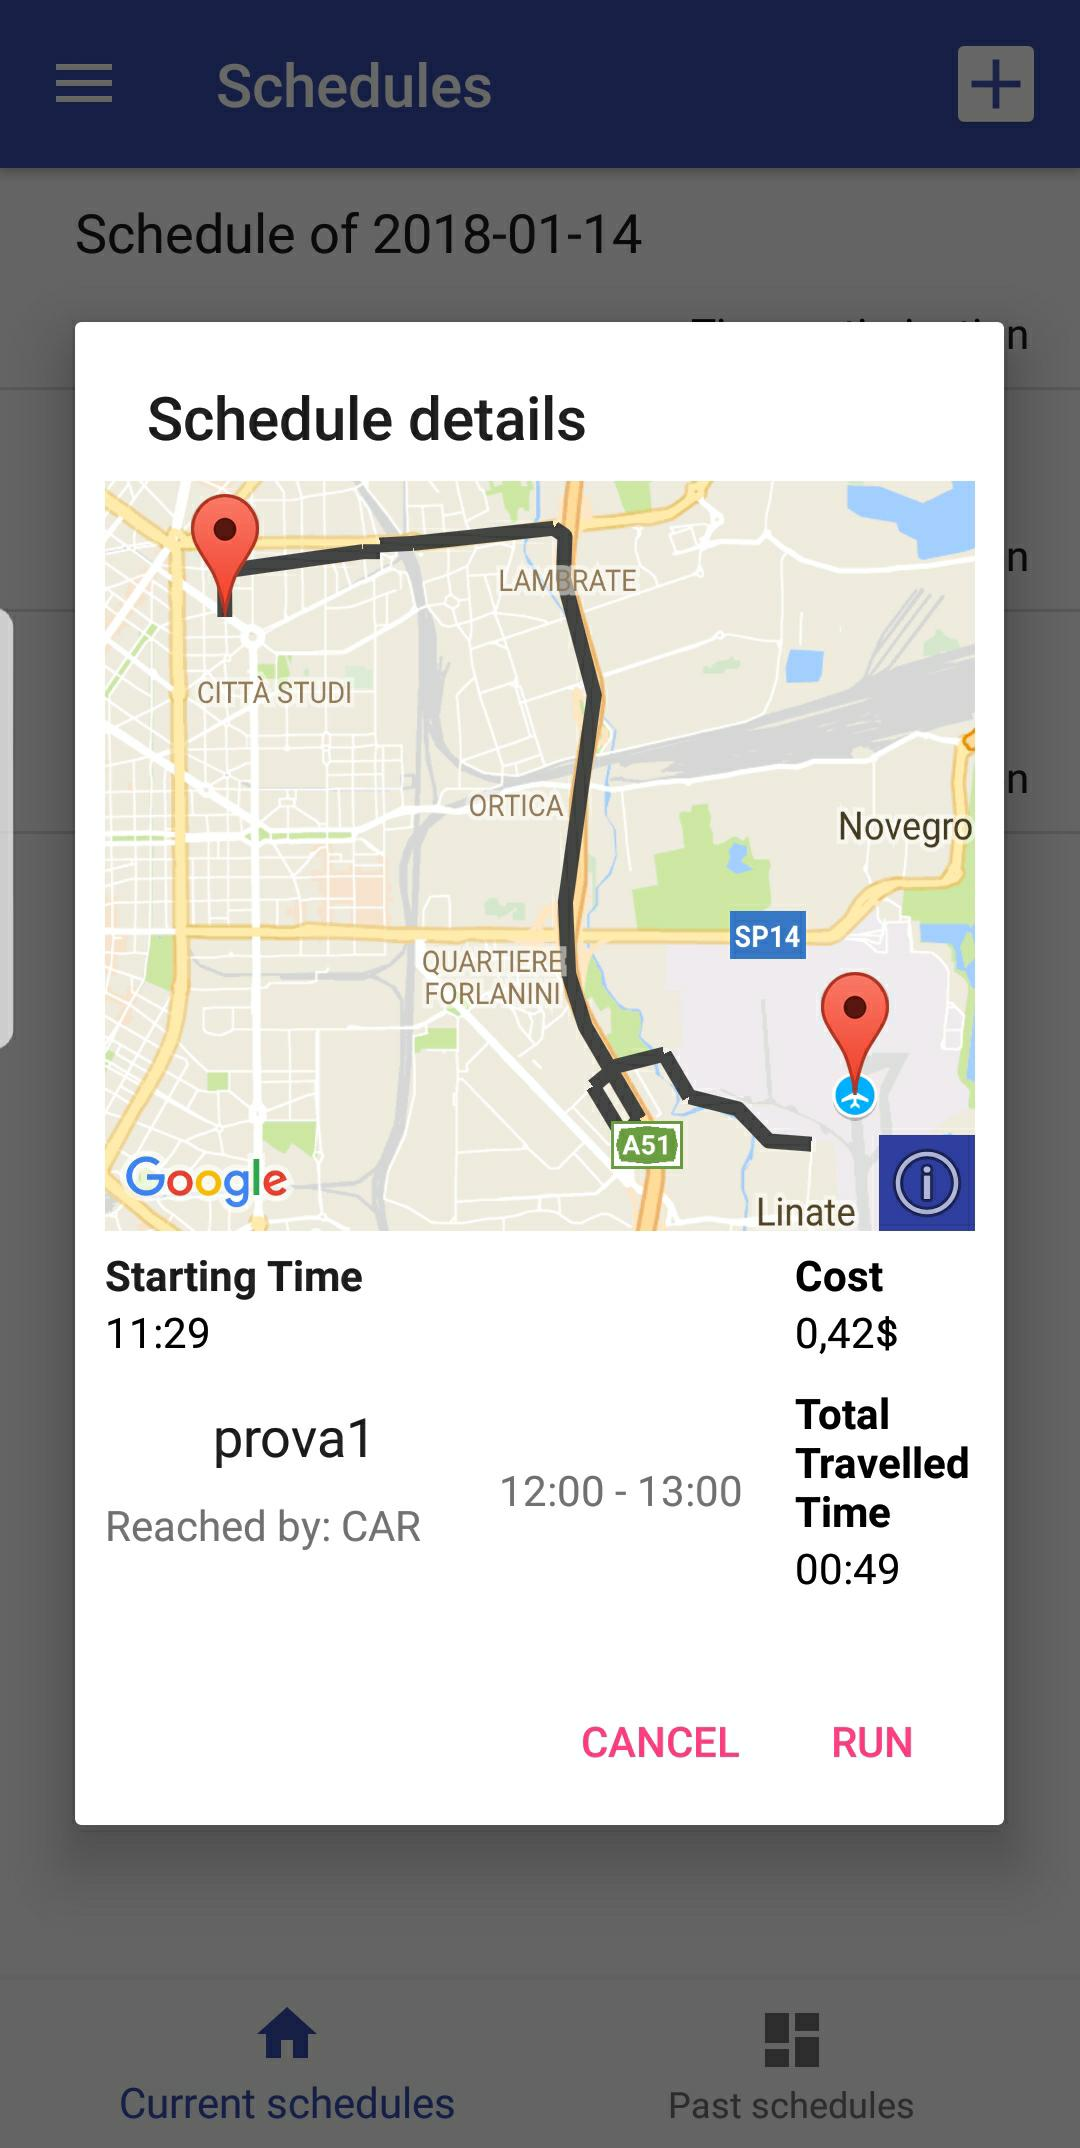
\includegraphics[width=0.2\linewidth]{Images/Goals/Car_route.jpg}
			\label{fig:CR}
			\end{center}
			\end{figure}			
			\subsubsection{Multiple Schedules}
			\begin{figure}[H]
			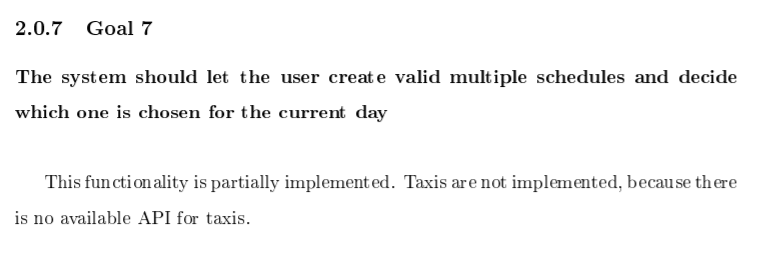
\includegraphics[width=\linewidth]{Images/Goals/Goal_7.png}
			\label{fig:G7}
			\end{figure}
			\paragraph{}The creation of the schedule sometimes doesn’t work properly. \\It can happen that the application sends an “infeasible schedule” notification without a clear reason (e.g.: wake up time: 7 a.m.; appointment time: 9 p.m. (distance of few km); optimization parameter: cost). Rarely, the application freezes on the “schedule creation” page. \\
When we were able to successfully create two schedules for the same day, this goal was reached correctly. 
			\subsubsection{Booking}
			\begin{figure}[H]
			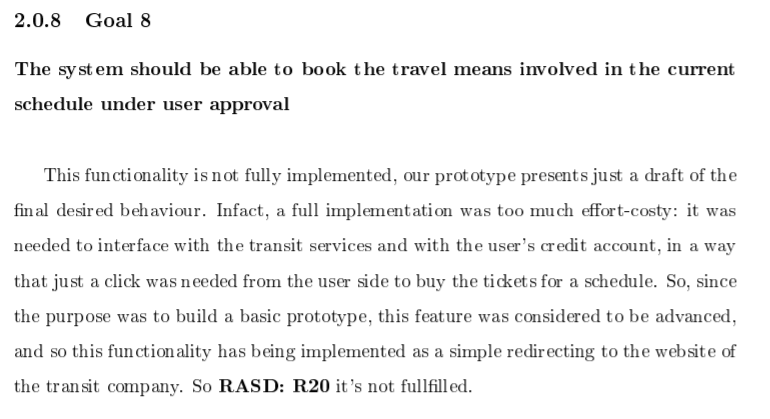
\includegraphics[width=\linewidth]{Images/Goals/Goal_8.png}
			\label{fig:G8}
			\end{figure}
			\paragraph{}We were not able to access this functionality. We tried to create multiple schedules in which we had to take public transports, but, after running the schedules, there wasn’t any redirection to the website of the transit company. We do not know if the application has this feature working, but we were not able to access it. 
			\subsubsection{Real Time User Position}
			\begin{figure}[H]
			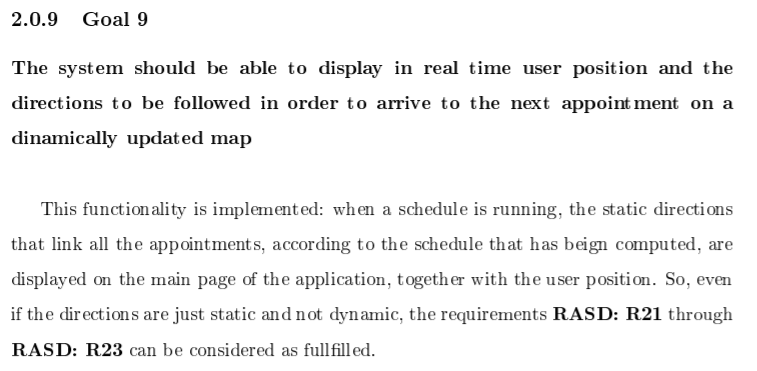
\includegraphics[width=\linewidth]{Images/Goals/Goal_9.png}
			\label{fig:G9}
			\end{figure}
			\paragraph{}This feature works as described above. Once the schedule is created, on the homepage of the application all the directions from the starting point to the location of the appointment are shown both on the map and as text on the bottom of the screen. The directions are well detailed and easy to follow.
			\subsubsection{Shared Travel Means}
			\begin{figure}[H]
			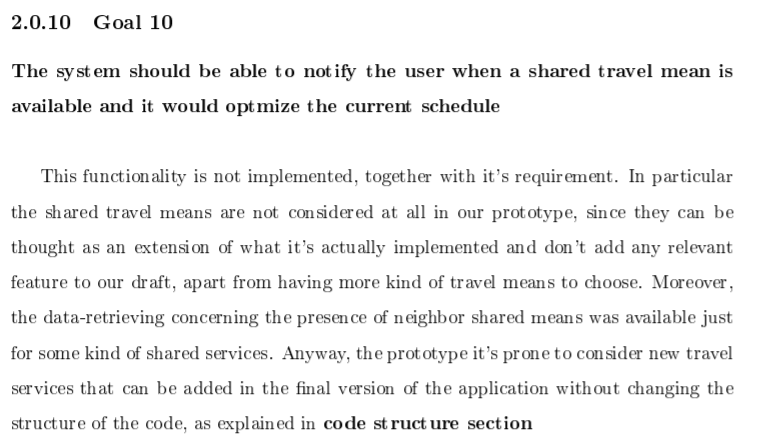
\includegraphics[width=\linewidth]{Images/Goals/Goal_10.png}
			\label{fig:G10}
			\end{figure}
			\paragraph{}This feature is not implemented.
\newpage
	\section{Final Conclusion}
		\paragraph{}The functionalities were well thought and accurately designed. However we found some problems while running the application. For example the application is not totally stable because some exceptions are not handled and, when you try to do some forbidden actions the system, instead of sending an error notification, will simply crash and you will lose all the temporary data.\\
Some of the options during  the creation of events and the schedule were not immediately comprehensible, for example while setting constraints for a schedule it asks you to input a max distance without specifying the measure unit.\\
We believe that these problems at the moment are not too concerning because it is simply a prototype, but should be fixed before the official launch of the application since they could generate frustration in the users and ruin their experience with this program.
\newpage
	\section{Effort Spent}
	\begin{itemize}
	\item{} Teamwork: 6 hours.
	\end{itemize}

\end{document}
